%UNIT 4: LINEAR DIFFERENTIAL EQUATIONS
%%%%%%%%%%%%%%%%%%%%%%%%%%%
%%%% Put the following at the top of each .tex file  %
\pagestyle{fancy}
\renewcommand{\theUnit}{2.3}
\ifthenelse{\isundefined{\UnitPageNumbers}}{}{\setcounter{page}{1}}
\rhead{Section \theUnit: Linear Differential Equations}
\lhead{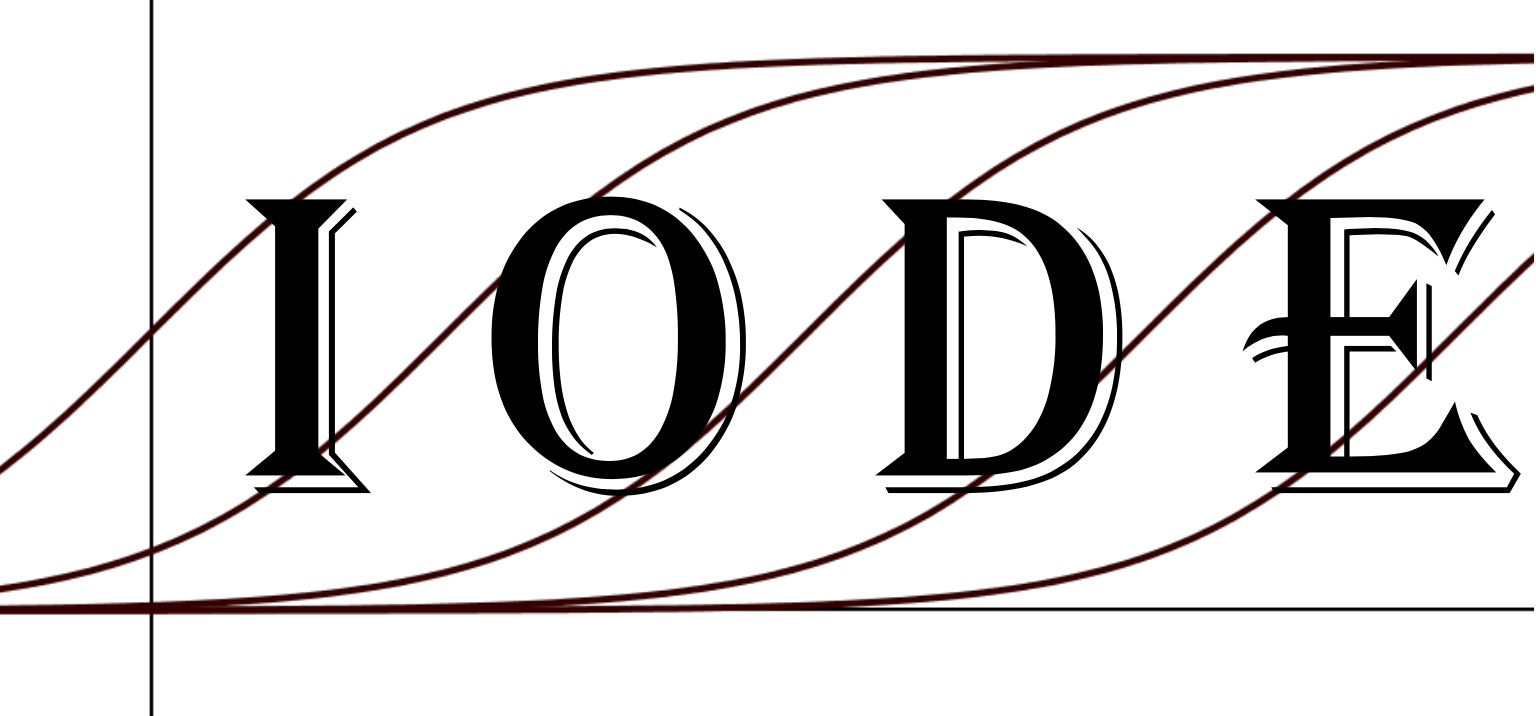
\includegraphics[width=1.25cm]{IODE-logo.png}}
\rfoot{\mypage}
\lfoot{}
\cfoot{}
\fancypagestyle{firstfooter}{\footskip = 50pt}
\renewcommand{\footrulewidth}{.4pt}
%%%%%%%%%%%%%%%%%%%%%%%%%%%
\vspace*{-20pt} \thispagestyle{firstfooter}
\pagebegin{A Salty Tank}
\begin{enumerate}
\item A very large tank initially contains 15 gallons of saltwater containing 6 pounds of salt. Saltwater containing 1 pound of salt per gallon is pumped into the top of the tank at a rate of 2 gallons per minute, while a well-mixed solution leaves the bottom of the tank at a rate of 1 gallon per minute. \label{06problem1}

\begin{enumerate}
\item Should the rate of change equation for this situation depend just on the amount of salt $S$ in the tank, the time $t$, or both $S$ and $t$? Explain your reasoning. \label{06problem1parta}
\vfill
\item The following is a general rule of thumb for setting up rate of change equations for situations like this where there is an input and an output: \label{06problem1partb}

\[\text{rate of change } = \text{ rate of change in } - \text{ rate of change out}\]

Using the above rule of thumb, figure out a rate of change equation for this situation. \\
{\em Hint}: Think about what the {\em units} of $\frac{dS}{dt}$ need to be, where $S$ is the amount of salt in the tank in pounds.
\vfill

\clearpage

\item	Use the slope field for this differential equation in the GeoGebra applet, \newline\href{https://ggbm.at/PFRcbkbZ}{\underline{https://ggbm.at/PFRcbkbZ}}, to sketch a graph of the solution with initial condition $S(0)=6$. Reproduce this sketch below. Estimate the amount of salt in the tank after 15 minutes. \label{06problem1partc} 
\end{enumerate}
\end{enumerate}

\vspace{-.5in}\hspace{-.1in}
\includegraphics[width=.5in]{06/06SaltyTankQR.png}
\vfill

\clearpage
 
The differential equation you developed for the salty tank is not separable, and therefore using the technique of separation of variables is not appropriate. This differential equation is  called \textbf{first order linear}, which means it has the form 
\[ a_1(x) \frac{dy}{dx}+ a_2(x) \cdot y=b(x),\]
where $a_1(x)$, $a_2(x)$, and $b(x)$ are all continuous functions of $x$ alone.
\vs
Note if we divide both sides by $a_1(x)$, we can rewrite any first order linear differential equation in \textbf{standard form}:
\[ \frac{dy}{dx} + P(x)y = Q(x).\]
\vs
The following technique, which we refer to as the \textbf{reverse product rule}, can be used find the general solution to a first-order linear equation.

\begin{enumerate}[resume]
\item Review the product rule as you remember it from calculus. In general symbolic terms, how do you represent the product rule? How would you describe it in words?
\vfill

Consider the differential equation $\displaystyle\frac{dy}{dx}+2y=3$. Note that this is a first order linear differential equation already in \textbf{standard form}, where $P(x)=2$ and $Q(x)=3$ are both continuous functions. The following illustrates a technique for finding the general solution to linear differential equations. The inspiration for the technique comes from a creative use of the product rule and the Fundamental Theorem of Calculus, as well as use of the previous technique of separation of variables.
\begin{center} \renewcommand{\arraystretch}{1.5}
\newcolumntype{V}{>{\arraybackslash} m{.6\linewidth} }
\begin{tabular}{|p{2.5in}|V|}
\hline
Use the product rule to expand $(y \mu)'$. & \begin{flushright}{\footnotesize Box 0}\end{flushright} \\
{} & {} \\ 
\hline
In the equation $\frac{dy}{dx}+2y=3$, rewrite $\frac{dy}{dx}$ as $y'$.& \begin{flushright}{\footnotesize Box 1}\end{flushright} \\
\hline
Notice that the left-hand side of the equation in Box 1 looks a lot like the expanded product rule but is missing the function $\mu$.  So multiply both sides by $\mu$, a function that we will determine shortly.  & \begin{flushright}{\footnotesize Box 2}\end{flushright} \\
\hline
Because, so far, $\mu$ is an arbitrary function, we can have $\mu$ satisfy any differential equation that we want. & \begin{flushright}{\footnotesize Box 3}\end{flushright} \\
Use $\mu' = 2\mu$ to rewrite the left-hand side of Box 2 to look like Box 0. & {} \\
\hline
%FORCE TABLE TO PAGEBREAK HERE
\end{tabular}\end{center}

\clearpage

\begin{center} \renewcommand{\arraystretch}{1.5}
\newcolumntype{V}{>{\arraybackslash} m{.6\linewidth} }
\begin{tabular}{|p{2.5in}|V|}
\hline
Use separation of variables to solve $\mu' = 2\mu$.   & \begin{flushright}{\footnotesize Box 4}\end{flushright} \\
{} & {} \\ 
{} & {} \\ 
\hline
Replace $\mu$ in the equation from Box 2 with your solution from Box 4. & \begin{flushright}{\footnotesize Box 5}\end{flushright} \\
{} & {} \\ 
\hline
Show that the equation in Box 5 can be rewritten as $\left(ye^{2x}\right)' = 3e^{2x}$ & \begin{flushright}{\footnotesize Box 6}\end{flushright} \\
{\em Hint}: Consider Box 0. & {} \\ 
{} & {} \\ 
\hline
Write integrals with respect to $x$ on both sides.  Apply the Fundamental Theorem of Calculus. & \begin{flushright}{\footnotesize Box 7}\end{flushright} \\
{} & {} \\ 
\hline
Obtain an explicit solution by isolating $y(x)$.& \begin{flushright}{\footnotesize Box 8}\end{flushright} \\
{} & {}\\
\hline
\end{tabular}
\end{center}

The key is finding a formula for the function $\mu(x)$ that we multiply on both sides which allowed us to ``reverse'' the product rule (going from Box 5 to Box 6). The function $\mu(x)$ is called the \textbf{integrating factor}. 
\bi
\ii Check that the differential equation is first order linear, and rewrite it in \textbf{standard form}:
\[ \frac{dy}{dx} + P(x)y = Q(x).\]
\ii Calculate the integrating factor: \vs
\[ \mu(x) = \ \ \ \ \ \ \ \ \ \ \ \ \ \ \ \ \ \ \ \ \ \ \ \ \ \ \ \ \ \ \ \ \ \ \ \ \ \ \ \ \mbox{(for convenience, set the abitrary constant $C=0$.)} \]
\ii Multiply both sides of the standard form by $\mu(x)$, and rewrite the equation as in Box 6:
\[ \frac{d}{dx} \left(y \mu(x) \right) = \mu(x) Q(x)\].
\ii Integrate both sides with respect to $x$, and solve for $y$ (if possible).
\ei

\clearpage

\item	Use the previous technique, which we refer to as the \textbf{method of integrating factors} or \textbf{reverse product rule}, to find the general solution for the Salty Tank differential equation from Problem \ref{06problem1}. \label{06problem3}
\vfill 

%\clearpage

\item \label{06problem4}
\begin{enumerate}
\item Use the general solution from problem \ref{06problem3} to find the particular solution corresponding to the initial condition $S(0) = 6$ and then use the particular solution to determine the amount of salt in the tank after 15 minutes. That is, compute $S(15)$. Your answer should be close to your estimate from problem \ref{06problem1partc}. Is it? If not, you likely made an algebraic error. \label{06problem4parta}
\vfill
\item What does your solution predict about the amount of salt in the tank in the long run?  How about the concentration? \label{06problem4partb}
\vfill
\item Explain how you can make sense of the predictions from \ref{06problem4partb} by using the differential equation itself. \label{06problem4partc}
\vfill
\end{enumerate}

%\end{enumerate}

\clearpage

%%% From AHS 18_Spring/Chap2/sec2-3

\ii Decide whether each differential equation is linear, and if so write it in standard form.
\bb
\ii $x^2y'=x^2-3y$ \vspace{1in}
\ii $2y \frac{dy}{dx} - 3y=8$ \vspace{1in}
\ee

\ii Solve the differential equation:
\bb
%\ii $\dsty x^2 \frac{dy}{dx}-xy=2x^3+x^2$  \vfill % $\mu(x)=\frac{1}{x}$, $y=2x^2+x\ln{(|x|)} + Cx$ 
\ii $\dsty z\frac{dw}{dz}+2w=5z^3$  \vfill % $\mu(z)= z^2$, $w=z^3+\frac{C}{w^2}$
\ii $\dsty \sin{x} \frac{dy}{dx} + y \cos{x} = x\sin{x}$, $y \left( \frac{\pi}{2} \right)=2$  \vfill %$\mu(x)=\sin{x}$, $y=-\frac{x\cos{x}}{\sin{x}}+1+\frac{1}{\sin{x}}$
%\ii $(1+t^2) \frac{dy}{dt} + 4ty=t$, $y \left( \frac{1}{2} \right) =16$  \vfill %$\mu(t)=(1+t^2)^2$, $y= \frac{\frac{1}{2}t^2+\frac{1}{4}t^4-2}{(1+t^2)^2}$  
\ee

\ee

\clearpage

%%%%%%%%%%%%%%%%%%%%%%%%%%%%%%%%%%%%%%%%
\pagebegin{Homework Set 4}

\begin{enumerate}
\item Find the general solutions to the following differential equations using separation of variables or the reverse product rule.  Give a reason as to why you used the method you chose over the other. \label{06HWproblem1}

\begin{enumerate}
\item $\displaystyle \frac{dy}{dt}=2y-t$
\item $\displaystyle \frac{dy}{dt}=-\frac{y}{t}+2$
\item $\displaystyle \frac{dy}{dt}=y\sin t$
\item $\displaystyle \frac{dy}{dt}=\cos t$	
\end{enumerate}

\item Solve the following differential equation in two ways: once using separation of variables, and once using the reverse product rule. \label{06HWproblem2} 
\[ \frac{dy}{dt} = 2y+1\, ; \quad y(0)=2\]

\item	For each of the following, determine which method(s) could be used to find the general solution. Do NOT actually find the general solutions, just determine any and all techniques that could be used. \label{06HWproblem3}

\begin{enumerate}
\item $\displaystyle \frac{dy}{dt}=2y-3e^{-t}$
\item $\displaystyle \frac{dy}{dt}=-0.2(75-y)$
\item $\displaystyle \frac{dy}{dt}=y^2+1$
\item $\displaystyle \frac{dy}{dt}=e^t y-\cos t$
\end{enumerate}

\item \label{06HWproblem4}
\begin{enumerate}
\item Create a differential equation (different from all those above) that can only be solved with separation of variables.
\item	Create a differential equation (different from all those above) that can only be solved with the reverse product rule method.
\item	Create a differential equation (different from all those above) that can be solved with either the reverse product rule method or separation of variables.
\end{enumerate}

\item	A tank initially contains 90 lb of salt dissolved in 20 gal of water. Brine containing 2 lb/gal of salt flows into the tank at the rate of 3 gal/min, and the mixture flows out of the tank at the same rate. How much salt does the tank contain 6 minutes later? \label{06HWproblem5}
\vfill

\clearpage

\item \label{06HWproblem6}
\begin{enumerate}
\item Use our technique for solving linear differential equations to verify that the exact solution to $\displaystyle\frac{dy}{dt}=2y-3e^{-t}$ with initial condition $y(0) = 1$ is $y(t) = e^{-t}$.

\item	Compare the long-term behavior of the exact solution and one or more tip to tail Euler's method approximations. Describe and graphically illustrate your results and develop an argument that explains or accounts for these results.

\item The Euler algorithm starts at some value, computes the rate of change at that value, and then assumes that this rate of change is going to be constant over a specified time interval. This process gets you to the next value and the entire process is repeated. In other words, for each time interval this recipe uses the rate of change at the beginning of each interval. One idea to improve this process is instead of using the value of the rate of change at the beginning of each time interval, calculate some sort of average of the rate of change values over the time interval and then use that averaged rate of change just as you would in the Euler recipe. Go to the library and look up in one or more differential textbooks the approximation method called Runge-Kutta. Write down what the algorithm for this method and briefly discuss why this method is better than the Euler method. 

\item	Use EXCEL to compare a Runge-Kutta approximation, an Euler's method approximation, and a graph of the exact solution for the differential equation $\displaystyle\frac{dy}{dt}=2y-3e^{-t}$ with initial condition $y(0) = 1$. Summarize your comparison below and discuss how (and why) the approximations differ from the graph of the exact solution.
\end{enumerate}

\item	Thus far in the course, we have approached analysis of rate of change equations in three different ways -- analytical approaches, numerical approaches, and graphical approaches. In words understandable to a calculus student planning to take differential equations, describe what it means to analytically, numerically, and graphically analyze solutions to a differential equation. Also, develop an explanation that would help this student understand when you might want to use one approach over the other and what advantages and disadvantages each accompanies each approach. \label{06HWproblem7}

\item	Some textbooks refer to the ``reverse product rule'' technique as the method of ``integrating factors.'' Do some research using the internet or textbooks and explain how the integrating factor method relates to the reverse product rule. \label{06HWproblem8}

\item Let's call the salty tank we discussed in class Tank A. \label{06HWproblem9} Consider the following modifications:
\begin{itemize}
\item Tank B is the same basic scenario as Tank A, but pure water is being pumped into Tank B instead of saltwater.
\item Tank C is the same  basic scenario as Tank A, but the rates are switched: saltwater enters Tank C at a rate of 1 gallon per minute, and leaves at a rate of 2 gallons per minute.
\item Tank D is the same  basic scenario as Tank A, but Tank D initially contains 6 gallons of pure water.
\end{itemize}
\begin{enumerate}
\item Set up and solve initial value problems that correspond to individual Tanks B, C, and D.
\item Use a plot to compare four solution curves and discuss how these curves predict/represent outcomes you might expect from the description of each scenario. 
\end{enumerate}

\item In this course so far we have discussed various analytic, numerical, and graphical methods and techniques for finding and understanding solutions to differential equations. Below are the methods discussed in this course, up to this point, in the left column. Match the technique to its appropriate category(ies), in the right column. \label{06HWproblem10}

\begin{center}
\begin{tabular}{lll}
\textbf{\underline{Technique}} & \hspace{2in} & \textbf{\underline{Category}} \\
& \hspace{2in} & \\
Euler's Method & \hspace{2in} & Analytic Technique \\
& \hspace{2in} & \\
Reverse Product Rule & \hspace{2in} & Numerical Technique \\
 &\hspace{2in} & \\
Slope Field & \hspace{2in} & Graphical Technique \\
& \hspace{2in} & \\
Separation of Variables & \hspace{2in} &
\end{tabular}
\end{center}


\end{enumerate}
